

\tikzset{every picture/.style={line width=0.75pt}} %set default line width to 0.75pt        

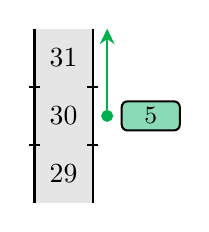
\begin{tikzpicture}[x=0.75pt,y=0.75pt,yscale=-0.7,xscale=0.7]
%uncomment if require: \path (0,300); %set diagram left start at 0, and has height of 300

%Shape: Rectangle [id:dp13563874266693043] 
\draw  [draw opacity=0][fill={rgb, 255:red, 0; green, 0; blue, 0 }  ,fill opacity=0.1 ] (230,60) -- (270,60) -- (270,180) -- (230,180) -- cycle ;
%Rounded Rect [id:dp5561959472232012] 
\draw  [fill={rgb, 255:red, 138; green, 218; blue, 184 }  ,fill opacity=1 ][line width=0.75]  (290,114) .. controls (290,111.79) and (291.79,110) .. (294,110) -- (326,110) .. controls (328.21,110) and (330,111.79) .. (330,114) -- (330,126) .. controls (330,128.21) and (328.21,130) .. (326,130) -- (294,130) .. controls (291.79,130) and (290,128.21) .. (290,126) -- cycle ;
%Straight Lines [id:da05571726881476602] 
\draw    (230,60) -- (230,180) (234,100) -- (226,100)(234,140) -- (226,140) ;
%Straight Lines [id:da7319727700794608] 
\draw    (270,60) -- (270,180) (274,100) -- (266,100)(274,140) -- (266,140) ;
%Straight Lines [id:da8116302583311774] 
\draw [color={rgb, 255:red, 0; green, 176; blue, 79 }  ,draw opacity=1 ]   (280,120) -- (280,63) ;
\draw [shift={(280,60)}, rotate = 90] [fill={rgb, 255:red, 0; green, 176; blue, 79 }  ,fill opacity=1 ][line width=0.08]  [draw opacity=0] (10.72,-5.15) -- (0,0) -- (10.72,5.15) -- (7.12,0) -- cycle    ;
\draw [shift={(280,120)}, rotate = 270] [color={rgb, 255:red, 0; green, 176; blue, 79 }  ,draw opacity=1 ][fill={rgb, 255:red, 0; green, 176; blue, 79 }  ,fill opacity=1 ][line width=0.75]      (0, 0) circle [x radius= 3.35, y radius= 3.35]   ;

% Text Node
\draw (250,80) node    {$31$};
% Text Node
\draw (250,119.5) node    {$30$};
% Text Node
\draw (310,120) node  [font=\small]  {${\textstyle 5}$};
% Text Node
\draw (250,160) node    {$29$};


\end{tikzpicture}
